\documentclass[a4j]{jarticle}
\usepackage{ascmac}
\usepackage[dvipdfmx]{graphicx}

\begin{document}

\title{計算機科学実験及演習1 報告書 \\ \bf 課題12}
% ↓ここに自分の氏名を記入
\author{安済 翔真}
\西暦
\date{提出日: \today} % コンパイル時の日付が自動で挿入される
\maketitle

\section{最短経路探索アルゴリズム}
\subsection{アルゴリズムの説明}
以下に、実装したダイクストラ法のアルゴリズムを示す。
\begin{enumerate}
  \item 距離が確定した頂点の集合A、始点から頂点vまでの距離を返す関数D(v)、
  最短経路において頂点vの1つ前に通る頂点を返す関数P(v)、少なくとも1回訪れた頂点の集合Q、
  頂点\(v, w\)間の辺の重みを返す関数\(W(v, w)\)を用意する。
  はじめは\(\forall v \in V(頂点全体の集合), D(v) = \infty \)としておく。
  \item 始点\(v_0\)からの距離\(D(v_0) = 0\)とする。また、Qに\(v_0\)を追加する。
  \item Qの要素数が0になるまで以下を繰り返す。
    \begin{enumerate}
      \item Qの要素の中で、始点からの距離が最小の要素vを取り出す。
      \item vに隣接する各頂点wに対して、\(D(w) > D(v) + W(v, w)\)ならば
      \(D(w) = D(v) + W(v, w)\)とし、\(Qにw\)を追加する。また、\(P(w) = v\)とする。
    \end{enumerate}
\end{enumerate}
以上の操作によって定められた\(P(v)\)の値を辿ることで始点から任意の点までの最短経路を求めることができる。

\newpage
\subsection{アルゴリズムの流れ図}
% 次の3行のコメントをはずし,図のファイル名,拡大縮小率を調整する.
\begin{figure}[h]
  \centering
  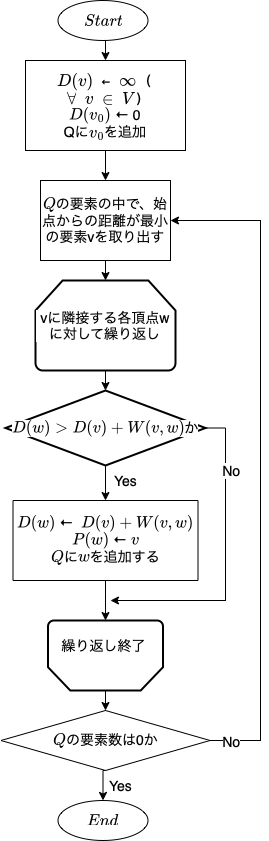
\includegraphics[scale=0.5]
    {report12.drawio.png}
\end{figure}

\subsection{実行例}
% MyGraphTestの典型的な実行例(端末からの入力や出力を含む)を示す.
% {screen}環境を使うと,枠を出力できる.

\begin{screen}
\$ java MyGraphTest \\
graph.txt  \\
3
\end{screen}

\section{クラス仕様}
% クラス仕様とは,そのクラスが持つ役割,
% メンバ変数,メソッドなどの仕様を記述したものである.
% 本レポートでは,自身が作成したクラス
%(MyGraphやMyEdgeなど)それぞれについて,
% subsectionを作成し,クラス仕様を記述すること

\subsection{Nodeクラス}

\subsubsection{役割}
% このクラスが持つ役割を簡潔に数行で記述する.
このクラスはグラフ内の辺を表す。辺の両端の頂点と辺の重みを変数として保持し、メソッドを呼び出すことで
それらを取得することができる。

\subsubsection{メンバ変数}
%クラスが持つすべてのメンバ変数について,descriptionで記述

\begin{description}
\item[Integer node1]
辺の両端の頂点のうち、頂点番号が小さい方の頂点の番号を保持する。

\item[Integer node2]
辺の両端の頂点のうち、頂点番号が大きい方の頂点の番号を保持する。

\item[Integer weight]
辺の重みを保持する。

\end{description}

%クラスが持つすべてのメソッドについて,subsubsectionを作り,説明
\subsubsection{getNodesメソッド}

\begin{description}
\item[機能]
辺の両端の頂点番号を配列として返す。

\item[インタフェース]\ \vspace{0mm}
\begin{enumerate}
  \item 引数: なし
  \item 用途: 辺の両端の頂点を取得する。
  \item 返り値の型: Integer[]
\end{enumerate}
\end{description}

\subsubsection{getWeight}

\begin{description}
\item[機能]
辺の両端の頂点番号を配列として返す。

\item[インタフェース]\ \vspace{0mm}
\begin{enumerate}
  \item 引数: なし
  \item 用途: 辺の重みを返す。
  \item 返り値の型: Integer[]
\end{enumerate}
\end{description}


\section{プログラムの評価}

% 以下のような点について自由記述.
% ・採用した設計,論理に関する検討(代替案との比較)
% ・プログラムの作成にあたって創意工夫した点
% ・テストの十分性(すべてのプログラムパスを網羅しているか)
% ・完成に至るまでに発生したバグの現象とその処置
% ・プログラムの機能的完成度(改良,拡張の余地)
% ・プログラムの効率
% ・その他


\section{プログラム開発の経過}

% プログラム開発の各段階で要した時間配分(工数)の概略を記す.
% あともどりがあった場合はその状況についても説明する.
% 各段階とは次の通り:
% 1. 問題の分析と解法の検討
% 2. クラス設計(クラスにどんなメソッドを用意するか設計すること)
% 3. クラス内論理設計/プログラミング(各メソッドを実際に実装すること)
% 4. プログラムテスト,デバッグ
% 5. 仕様書の作成(このレポートの作成)

\section{感想}

% 自由記述.
% シラバスに示した参考書以外のものを参照した場合,それも記す.

\newpage
\section*{付録}

% 作成したすべてのクラスのソースコードをつける.
% \ver

\end{document}
